\documentclass[]{article}
\usepackage[
            left=1in,right=1in,top=1in,bottom=1in,%
            footskip=.25in]{geometry}
\usepackage{enumitem}
\usepackage{array}
\usepackage{amsmath}
\usepackage{amssymb}
\usepackage{graphicx}
\usepackage{verbatim}
\usepackage{hyperref}
\usepackage{subcaption}
\usepackage{physics}
\usepackage{mwe}
\usepackage{graphicx}
\usepackage{pbox}
\usepackage{multicol}
\usepackage[utf8]{inputenc}
\hypersetup{
    colorlinks=true,
    linkcolor=blue,
    filecolor=magenta,      
    urlcolor=cyan,
}

\setlength{\arrayrulewidth}{0.2mm}
\setlength{\tabcolsep}{5pt}
\renewcommand{\arraystretch}{1.5}
\newcolumntype{L}{>{$}c<{$}}


%opening
\title{Causal Inference with Complex Dynamical Systems}
\author{George Stepaniants}

\begin{document}

\maketitle
\begin{abstract}
We review in this paper the definitions of Granger Causality and Convergent Cross Mappings (CCM). We show that their application to linear and nonlinear physical oscillator systems fail to reproduce accurate network reconstructions. We find a regime that involves perturbing and heavily damping these systems under which both methods give back the correct network topologies. A perturbation based network inference approach is presented to solve this problem. It is evaluated on simulated data from systems of linear and nonlinear connected oscillators. Reasoning behind this method is discussed.
\end{abstract}

\section{Introduction and Overview}


\section{Causal Inference Methods}
\subsection{Granger Causality}

\subsection{Convergent Cross Mapping}

\subsection{Perturbation Inference}


\section{Oscillator Systems}
\subsection{Harmonic Oscillators}
The standard equation for a damped harmonic oscillator is
\begin{align*}
\frac{d^2x}{dt^2} = 
\end{align*}


The first system we investigate is that of $n$ coupled harmonic oscillators where $\mathbf{x}$ is the vector of displacements of all oscillators. This network of oscillators has fixed boundary conditions so oscillator 1 and oscillator $n$ are attached to walls by springs. Also, pairs of oscillators in the network are connected to each other by springs with varying spring constants. Strength of coupling between oscillators and walls in this network is denoted by the $n + 1 \times n + 1$ matrix of spring constants
\begin{align*}
a
\end{align*}

Note that in a physical system of harmonic oscillators, the coupled interactions between pairs of oscillators are symmetric so the spring constant $A_{ij}$ from oscillator $i$ to oscillator $j$ is equal to the spring constant $A_{ji}$ from oscillator $j$ to oscillator $i$. Therefore, in this system the matrix $A$ is symmetric. The vector $\mathbf{m}$ contains the masses of all harmonic oscillators in this system and $c$ is the scalar damping coefficient.

A picture of a possible network configuration is shown in Figure [?]. The system of ODEs that governs the movement of these oscillators is
\begin{align*}
\mathbf{m} \cdot \frac{d^2\mathbf{x}}{dt^2} = A\mathbf{x} - c\frac{d\mathbf{x}}{dt}
\end{align*}

\subsection{Directed Harmonic Oscillators}

\subsection{Kuramoto Oscillators}


\section{Numerical Experiments}
Used MVGC toolbox for GC. Used R toolbox for CCM.


\section{Computational Results}
\subsection{Inference for Two Oscillator System}
Figure 1 shows the confusion matrix for GC inference over all possible directed networks of two harmonic or Kuramoto oscillators. As we can see, GC systematically predicts that all two oscillator networks are fully connected.

Figure 2 shows the confusion matrix for CCM inference over all possible directed networks of two harmonic or Kuramoto oscillators. As we can see, CCM systematically predicts that all two oscillator networks are fully connected.

Figure 3 shows the confusion matrix for PC inference over all possible directed networks of two harmonic or Kuramoto oscillators with one node perturbed.

Figure 4 shows the confusion matrix for PC inference over all possible directed networks of two harmonic or Kuramoto oscillators with both nodes perturbed.

The performance of PC is shown for different combinations of network connection probabilities and spring constants in Figure 5.

\begin{figure}
    \centering
    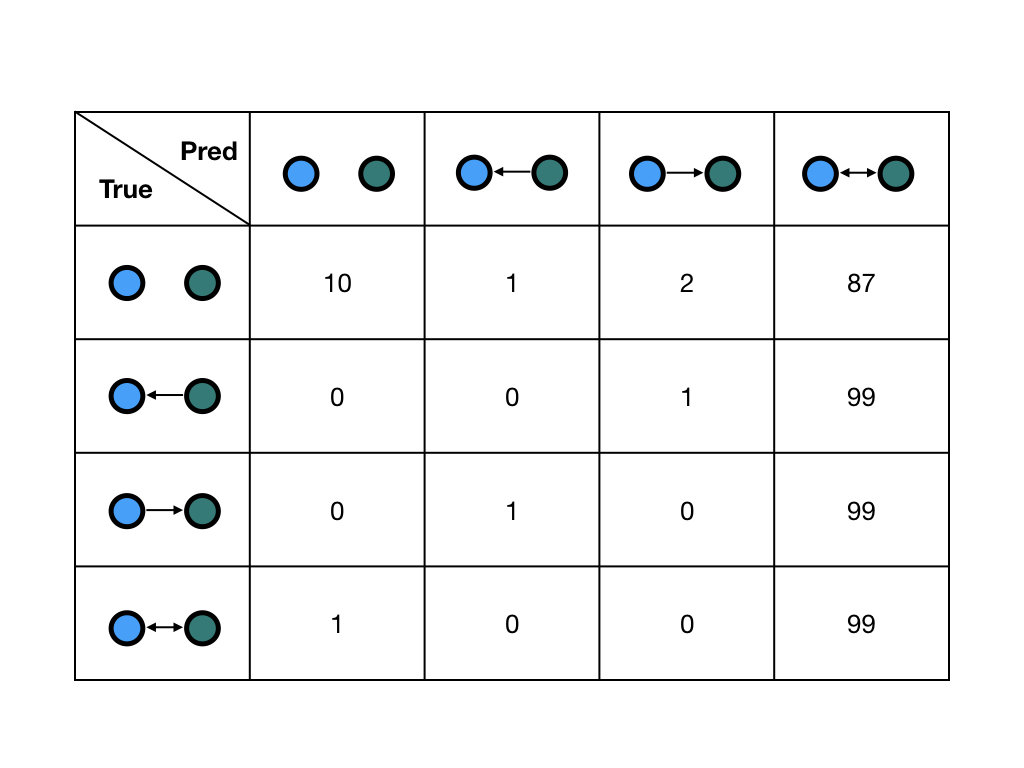
\includegraphics[width=12cm]{GrangerConfusionMatrix.jpeg}
    \caption{Confusion matrix for GC on networks of two oscillators.}
    \label{fig:example}
\end{figure}

\begin{figure}
    \centering
    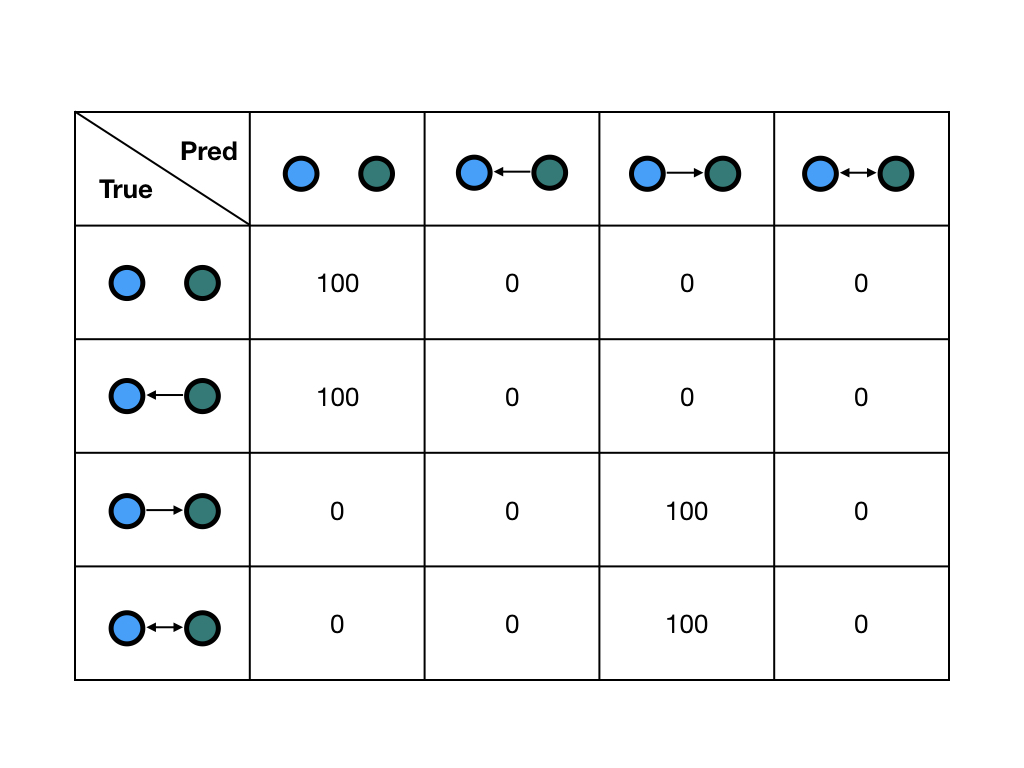
\includegraphics[width=12cm]{Pert1ConfusionMatrix.jpeg}
    \caption{Confusion matrix for PC on networks of two oscillators with all nodes observed and only blue node perturbed.}
    \label{fig:example}
\end{figure}

\begin{figure}
    \centering
    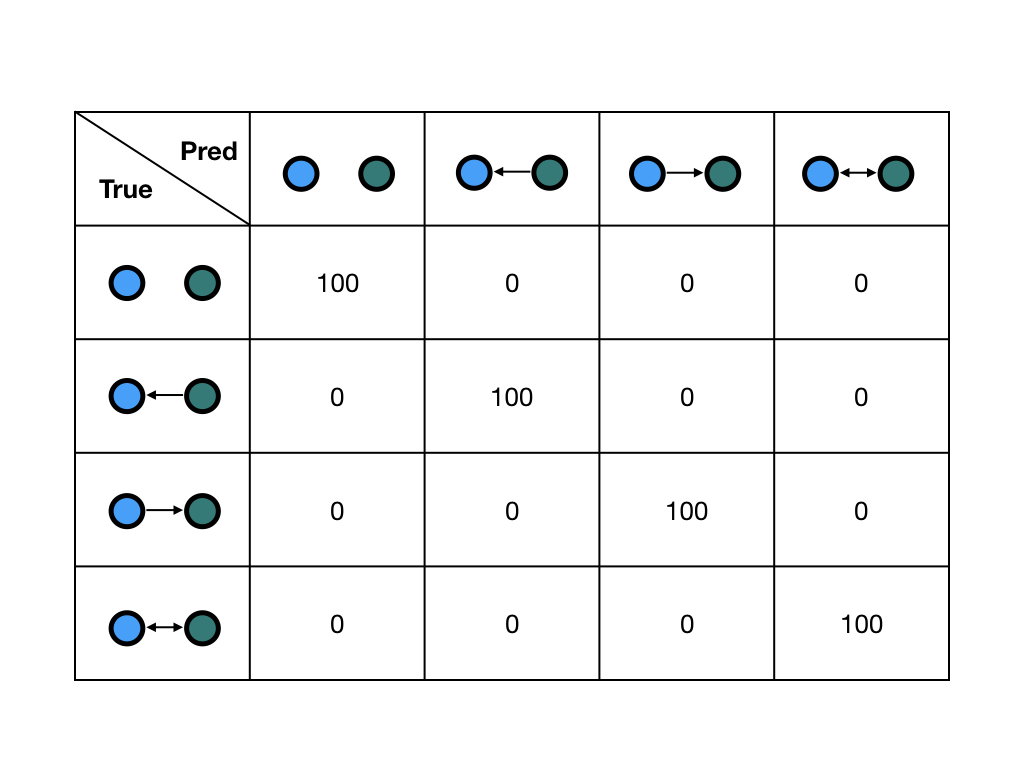
\includegraphics[width=12cm]{Pert2ConfusionMatrix.jpeg}
    \caption{Confusion matrix for PC on networks of two oscillators with all nodes observed and perturbed.}
    \label{fig:example}
\end{figure}

\subsection{Inference for N Oscillators}
Give statistics like accuracy, TPR, FPR over different simulations of N oscillators. Don't damp or do anything special with the simulation parameters.

\subsection{Inference with Damped Oscillator System}
Give statistics like accuracy, TPR, FPR over different simulations of N oscillators.


\section{Analysis}
\subsection{Reasons why Granger Causality Fails for Harmonic Oscillator Systems}


% Tables for all experiments
\clearpage
\begin{table}
\tiny
\begin{tabular}{| c | L | c | L | L | L | L | L | c | L | L | L | L | c | L |}
\hline
\multicolumn{15}{|c|}{Summary of GC Experiments for Harmonic Oscillators} \\
\hline
\hline
\textbf{Experiment Name} & \mathbf{n} & $\mathbf{A}$ & \mathbf{K} & \mathbf{m} & \mathbf{p_0} & \mathbf{v_0} & \mathbf{\gamma} & \textbf{Forcing} & \mathbf{N} & \mathbf{\Delta t} & \mathbf{T} & \mathbf{s} & \textbf{Prep} & \textbf{Reps} \\
\hline
gcH1 & 2 & All four two-node networks & 0.1, 0.2, ..., 10 & 1 & [-0.5, 0.5] & 0 & 0 & None & 100 & 0.1 & 25 & 0.1 & Detrend & 1 \\
\hline
gcH5 (deviate with small mass) & 5 & ER $p=0.5$ & 1 & ^a & ^b & 0 & 0 & None & 100 & 0.1 & 25 & 0.1 & Detrend & 1 \\
\hline
gcH6 (deviate with large damping, show diff K) & 5 & ER $p=0.5$ & 0.1, 0.2, ..., 10 & 1 & ^b & 0 & 10 & None & 100 & 0.1 & 25 & 0.1 & Detrend & 1 \\
\hline
\end{tabular}
\\[1cm]


\begin{tabular}{| c | L | c | L | L | L | L | c | L | L | L | L | c | L |}
\hline
\multicolumn{14}{|c|}{Summary of GC Experiments for Kuramoto Oscillators} \\
\hline
\hline
\textbf{Experiment Name} & \mathbf{n} & $\mathbf{A}$ & \mathbf{K} & \mathbf{\theta_0} & \mathbf{\omega} & \mathbf{\gamma} & \textbf{Forcing} & \mathbf{N} & \mathbf{\Delta t} & \mathbf{T} & \mathbf{s} & \textbf{Prep} & \textbf{Reps} \\
\hline
gcK1 & 2 & All four two-node networks & 0.1, 0.2, ..., 10 & [0, 2\pi] & [-1, 1] & 0 & None & 100 & 0.1 & 25 & 0.1 & Detrend & 1 \\
\hline
gcH6 (deviate with large damping, show diff K) & 5 & ER $p=0.5$ & 0.1, 0.2, ..., 10 & [0, 2\pi] & [-1, 1] & 10 & None & 100 & 0.1 & 25 & 0.1 & Detrend & 1 \\
\hline
\end{tabular}
\\[1cm]


\begin{tabular}{| c | L | c | L | L | L | L | L | c | L | L | L | L | c | L |}
\hline
\multicolumn{15}{|c|}{Summary of CCM Experiments for Harmonic Oscillators} \\
\hline
\hline
\textbf{Experiment Name} & \mathbf{n} & $\mathbf{A}$ & \mathbf{K} & \mathbf{m} & \mathbf{p_0} & \mathbf{v_0} & \mathbf{\gamma} & \textbf{Forcing} & \mathbf{N} & \mathbf{\Delta t} & \mathbf{T} & \mathbf{s} & \textbf{Prep} & \textbf{Reps} \\
\hline
ccmH1 & 2 & All four two-node networks & 0.1, 0.2, ..., 10 & 1 & [-0.5, 0.5] & 0 & 0 & None & 100 & 0.1 & 25 & 0.1 & Detrend & 1 \\
\hline
ccmH5 (deviate with small mass) & 5 & ER $p=0.5$ & 1 & ^a & ^b & 0 & 0 & None & 100 & 0.1 & 25 & 0.1 & Detrend & 1 \\
\hline
ccmH6 (deviate with large damping, show diff K) & 5 & ER $p=0.5$ & 0.1, 0.2, ..., 10 & 1 & ^b & 0 & 10 & None & 100 & 0.1 & 25 & 0.1 & Detrend & 1 \\
\hline
\end{tabular}
\\[1cm]


\begin{tabular}{| c | L | c | L | L | L | L | c | L | L | L | L | c | L |}
\hline
\multicolumn{14}{|c|}{Summary of CCM Experiments for Kuramoto Oscillators} \\
\hline
\hline
\textbf{Experiment Name} & \mathbf{n} & $\mathbf{A}$ & \mathbf{K} & \mathbf{\theta_0} & \mathbf{\omega} & \mathbf{\gamma} & \textbf{Forcing} & \mathbf{N} & \mathbf{\Delta t} & \mathbf{T} & \mathbf{s} & \textbf{Prep} & \textbf{Reps} \\
\hline
ccmK1 & 2 & All four two-node networks & 0.1, 0.2, ..., 10 & [0, 2\pi] & [-1, 1] & 0 & None & 100 & 0.1 & 25 & 0.1 & Detrend & 1 \\
\hline
ccmH6 (deviate with large damping, show diff K) & 5 & ER $p=0.5$ & 0.1, 0.2, ..., 10 & [0, 2\pi] & [-1, 1] & 10 & None & 100 & 0.1 & 25 & 0.1 & Detrend & 1 \\
\hline
\end{tabular}
\\[1cm]


\begin{tabular}{| c | L | L | L | c | L | L | L | L | L | c | L | L | L | L | c |}
\hline
\multicolumn{14}{|c|}{Summary of PC Experiments for Harmonic Oscillators} \\
\hline
\hline
\textbf{Experiment Name} & \mathbf{n} & \mathbf{n_\text{pert}} & \mathbf{n_\text{obs}} & $\mathbf{A}$ & \mathbf{K} & \mathbf{m} & \mathbf{p_0} & \mathbf{v_0} & \mathbf{\gamma} & \textbf{Forcing} & \mathbf{N} & \mathbf{\Delta t} & \mathbf{T} & \mathbf{s} & \textbf{Method} \\
\hline
pcH1 & 2 & 1, 2 & 1, 2 & All four two-node networks & 0.1, 0.2, ..., 10 & 1 & [-0.5, 0.5] & [-1, 1] & 0.1 & None & 100 & 0.1 & 25 & 0.1 & corr \\
\hline
pcH1 & 2 & 1, 2 & 1, 2 & All four two-node networks & 0.1, 0.2, ..., 10 & 1 & [-0.5, 0.5] & [-1, 1] & 0.1 & None & 100 & 0.1 & 25 & 0.1 & chngpt \\
\hline
pcH10 & 10 & 1, 2, ..., 10 & 10 & ER $p=0.1, 0.2, ..., 1$ & 1 & 1 & [-0.5, 0.5] & [-1, 1] & 0.3 & Pulse$^b$ & 10 & 0.1 & ^c & 0.1 & corr \\
\hline
pcH20 & 20 & 1, 2, ..., 20 & 1, 2, ..., 20 & ER $p=0.5$ & 0.1 & 1 & [-0.5, 0.5] & [-1, 1] & 0.3 & Pulse$^b$ & 10 & 0.1 & ^c & 0.1 & corr \\
\hline
pcH21 & 20 & 1, 2, ..., 20 & 1, 2, ..., 20 & BA $m=10$ & 0.1 & 1 & [-0.5, 0.5] & [-1, 1] & 0.3 & Pulse$^b$ & 10 & 0.1 & ^c & 0.1 & corr \\
\hline
\end{tabular}
\\[1cm]


\begin{tabular}{| c | L | L | L | c | L | L | L | L | c | L | L | L | L | c |}
\hline
\multicolumn{15}{|c|}{Summary of PC Experiments for Kuramoto Oscillators} \\
\hline
\hline
\textbf{Experiment Name} & \mathbf{n} & \mathbf{n_\text{pert}} & \mathbf{n_\text{obs}} & $\mathbf{A}$ & \mathbf{K} & \mathbf{\theta_0} & \mathbf{\omega} & \mathbf{\gamma} & \textbf{Forcing} & \mathbf{N} & \mathbf{\Delta t} & \mathbf{T} & \mathbf{s} & \textbf{Method} \\
\hline
pcK1 & 2 & 1, 2 & 1, 2 & All four two-node networks & 0.1, 0.2, ..., 10 & [0, 2\pi] & [-1, 1] & 0 & None & 100 & 0.1 & 25 & 0.1 & meanvar \\
\hline
pcK1 & 2 & 1, 2 & 1, 2 & All four two-node networks & 0.1, 0.2, ..., 10 & [0, 2\pi] & [-1, 1] & 0 & None & 100 & 0.1 & 25 & 0.1 & chngpt \\
\hline
pcK20 & 20 & 1, 2, ..., 20 & 1, 2, ..., 20 & ER $p=0.5$ & 0.1 & [0, 2\pi] & [-1, 1] & 0 & Pulse$^b$ & 10 & 0.1 & ^c & 0.1 & meanvar \\
\hline
pcK21 & 20 & 1, 2, ..., 20 & 1, 2, ..., 20 & BA $m=10$ & 0.1 & [0, 2\pi] & [-1, 1] & 0 & Pulse$^b$ & 10 & 0.1 & ^c & 0.1 & meanvar \\
\hline
\end{tabular}\\

\footnotesize{
$^a$ Make one mass very small compared to the rest\\
$^b$ Displace only one mass from equilibrium\\
$^b$ Short pulses of force for each perturbation\\
$^c$ $T$ changes in size to fit all perturbations in simulation
}
\end{table}


\clearpage
\section{Appendix A}
\subsection{Calculating Wait Time for Damped Harmonic Oscillators}
Our perturbation approach requires that the forcing perturbation in the oscillator system decays to zero before the next forcing perturbation can be applied. This requires that we calculate a wait time between perturbations for every simulation. Below we discuss how this wait time is computed for the case of coupled harmonic oscillators. The general equation for a harmonic oscillator network is
\begin{align*}
\frac{d^2\mathbf{x}}{dt^2} + c\frac{d\mathbf{x}}{dt} - M\mathbf{x} = \mathbf{F}(t)
\end{align*}
where the displacements $\mathbf{x}$ and forcing function $\mathbf{F}$ are vectors of length $n$. In our simulations, we make our forcing function be a step function of the form
\begin{align*}
\mathbf{F}(t) = \begin{array}{cc}
  \Big\{ & 
    \begin{array}{cc}
      \mathbf{0} & t < t_0 \\
      \mathbf{f}  & t_0 \leq t \leq t_0 + \Delta t \\
      \mathbf{0} & t > t_0 + \Delta t
    \end{array}
\end{array}
\end{align*}
where $t_0$ is the time of the perturbation and $\Delta t$ is the length of time under which the system is forced.

To solve this equation, let's first solve the homogeneous equation
\begin{align*}
\frac{d^2\mathbf{x}}{dt^2} + c\frac{d\mathbf{x}}{dt} - M\mathbf{x} = 0
\end{align*}
This equation has $n$ linearly independent solutions of the form $\mathbf{x}_i(t) = \mathbf{v}_ie^{\omega_i t}$ for $1 \leq i \leq n$. Substituting $\mathbf{x}_i$ into the homogeneous equation we have
\begin{align*}
(\omega_i^2 + c\omega_i - M)\mathbf{v}_i = 0
\end{align*}

This implies that $M\mathbf{v}_i = (\omega_i^2 + c\omega_i)\mathbf{v_i}$ so $\mathbf{v}_i$ is an eigenvector of $M$ with eigenvalue $\lambda_i = \omega_i^2 + c\omega_i$. Solving the quadratic equation for $\omega_i$, we have that
\begin{align*}
\omega_i = \frac{-c \pm \sqrt{c^2 + 4\lambda_i}}{2}
\end{align*}

Now note that if $w_i$ has a positive real part, then our solution to this differential equation will diverge. This agrees with experimental simulations. !!!Not sure how to deal with $\pm$ in quadratic equation solution so just taking plus here!!!

Now let's assume that $\Re(w_i) < 0$ for all $1 \leq i \leq n$. Using our forcing function $\mathbf{F}(t)$ defined above, let's solve our differential equation in the time $t \in [t_0, t_0 + \Delta t]$. In this time interval, $\mathbf{F}(t) = \mathbf{f}$ for some constant $f \in \mathbb{R}^n$ so
\begin{align*}
\frac{d^2\mathbf{x}}{dt^2} + c\frac{d\mathbf{x}}{dt} - M\mathbf{x} = \mathbf{f}
\end{align*}

If $\mathbf{x}_{hom}$ is the homogeneous solution to the equation above, then as long as the matrix $M$ is invertible, the general solution to our ODE is
\begin{align*}
\mathbf{x} = \mathbf{x}_{hom} - M^{-1}\mathbf{f}
\end{align*}

This indeed agrees with our simulations as on this time interval when forcing is applied, each $i$th node's trajectory oscillates about $(-M^{-1}\mathbf{f})_i$. Now, after time $t_0 + \Delta t$, the forcing stops and $\mathbf{F}(t) = \mathbf{0}$. At time $t = t_0 + \Delta t$, on average our oscillators have positions $\mathbf{x}(t_0 + \Delta t) = -M^{-1}\mathbf{f}$ and now their trajectories are once again dictated by the solution of the homogenous equation. So now we want to solve the ODE
\begin{align*}
\frac{d^2\mathbf{x}}{dt^2} + c\frac{d\mathbf{x}}{dt} - M\mathbf{x} = 0
\end{align*}
on the interval $t \in [t_0 + \Delta t, \infty)$ where $\mathbf{x}(t_0 + \Delta t) = -M^{-1}\mathbf{f}$. For simplicity, we can imagine that we are solving this problem on the time interval $t \in [0, \infty)$ with initial conditions $\mathbf{x}(0) = -M^{-1}\mathbf{f}$.

We would like to compute an upper bound for the amount of time it would take the magnitude of our solution to decay to $\epsilon > 0$. Writing out the general form of the solution we have
\begin{align*}
\mathbf{x}(t) = \sum_{i=1}^n \mathbf{x}_i(t) = \sum_{i=1}^n \mathbf{v}_ie^{\omega_i t}, \quad \mathbf{x}(0) = -M^{-1}\mathbf{f}
\end{align*}

Now we want to find a time $t_{wait}$ so that for all $t > t_{wait}$ we have $||\mathbf{x}(t)|| < \epsilon$. Taking the magnitude of our solution
\begin{align*}
||\mathbf{x}(t)|| = ||\sum_{i=1}^n \mathbf{v}_ie^{\omega_i t}||
\end{align*}
But note that all the eigenvectors $\mathbf{v}_i$ are mutually orthogonal so
\begin{align*}
||\mathbf{x}(t)|| = \sum_{i=1}^n ||\mathbf{v}_ie^{\omega_i t}|| \leq \sum_{i=1}^n ||\mathbf{v}_i|| e^{\Re(\omega_i)t}
\end{align*}

We also know from our initial conditions that the magnitudes of the eigenvectors $v_i$ are chosen such that $\mathbf{x}(0) = \sum_{i=1}^n \mathbf{v}_i = -M^{-1}\mathbf{f}$ which implies that $\sum_{i=1}^n ||\mathbf{v}_i|| = ||M^{-1}\mathbf{f}||$. If $\omega_{max}$ is the frequency with the largest (nonpositive) real part, we can write out
\begin{align*}
\sum_{i=1}^n ||\mathbf{v}_i|| e^{\Re(\omega_i)t} \leq ||M^{-1}\mathbf{f}||e^{\Re(\omega_{max})t} < \epsilon
\end{align*}

So for all $t > \frac{\log(\epsilon / ||M^{-1}\mathbf{f}||)}{\Re(\omega_{max})}$, we have that $||\mathbf{x}(t)|| < \epsilon$. Therefore, the wait time between perturbations for a network of damped harmonic oscillators is
\begin{align*}
t_{wait} = \frac{\log(\epsilon / ||M^{-1}\mathbf{f}||)}{\Re(\omega_{max})}
\end{align*}

\section{Appendix B}


\begin{thebibliography}{9}
\bibitem{1}

\bibitem{2}

\end{thebibliography}

\end{document}
